\headerbox{BuS framework and posterior sampling}{name=bus,span=2,column=1,row=0}{
%\headerbox{BuS framework}{name=bus,column=0,row=0,below=problem}{
%Introduced by \cite{bus}, the Bayesian update Structural Reliability (BuS) framework casts Bayesian inversion into an equivalent Structural Reliability (SR) problem.
%\par\noindent
By considering $P \sim \mathcal{U}(0,1)$ and the joint random variables $(P, \vec{X})$, one defines the limit state function $h : [0,1] \times \Dx \rightarrow \R$ which usually corresponds in SR to the difference between a resistance (R) contribution and a stress (S) contribution.
{\smaller
$$
h(p, \vec{x}) = R(p) - S(\vec{x}) = p - c \Lk(\vec{x};\vec{y}), \quad
c > 0
$$
}
%In SR, the failure domain $F$ it's characterized by $h(p, \vec{x}) \le 0$ and the failure probability $\mathbb{P}_f$ is the probability associated to $F$.
%\par\noindent
BuS rewrites the posterior distribution in terms of a marginal probability over the failure domain $F$
{\smaller
$$
\pi(\vec{x}|\vec{y}) = \frac{\pi(\vec{x})}{c\mathcal{Z}} \int_0^{c\Lk(\vec{x};\vec{y})}  dp = \frac{1}{\mathbb{P}(F)} \int_0^1 \mathbbm{1}_F(p, \vec{x}) \pi(\vec{x}) dp, \quad
F \stackrel{\text{def}}{=} \{(p,\vec{x}) : h(p, \vec{x}) \le 0\}
$$
}

%Subset Simulation (SuS) \cite{sus} is suitable for the efficient estimation of small probabilities, such as the failure probability of SR problems. 
Subset Simulation is adopted for the sampling procedure of posterior $(P, \vec{X})$:
{\smaller
$$
\pi(p,\vec{x}|F) = \pi(p,\vec{x}|F_{r+1}) \propto \mathbbm{1}_{F_{r+1}}(p,\vec{x}) \pi(\vec{x})
$$
}
\begin{center}
\begin{minipage}{0.85\textwidth}
\centering
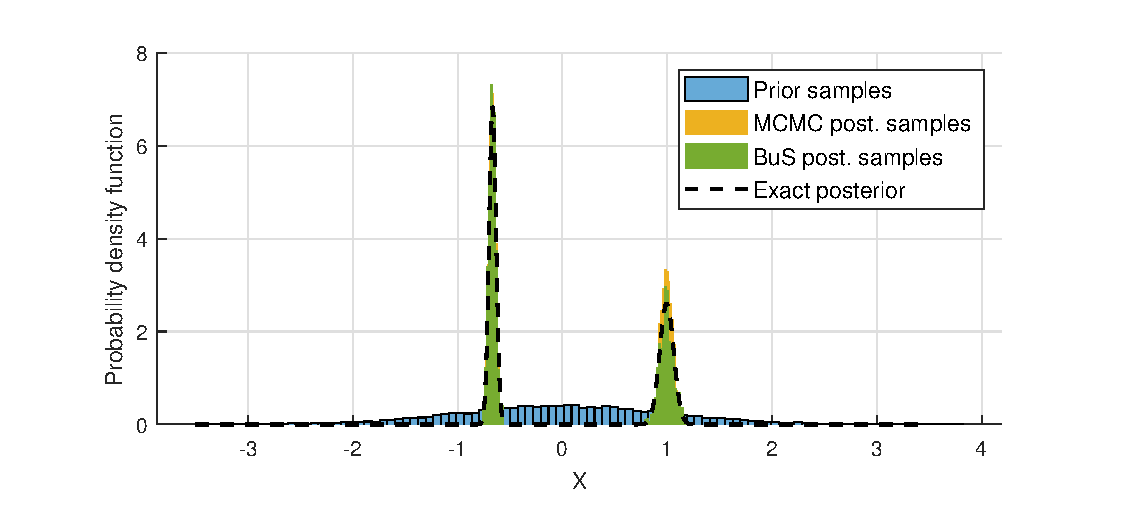
\includegraphics[width=0.75\textwidth]{post_apocalyptic.eps}
\captionof*{figure}{BuS-SuS posterior distribution compared to the exact posterior distribution and a classical MCMC approach sampling for a specific two-peaked test case of Bayesian inversion.}
\end{minipage}
\end{center}
}